\documentclass{article}
\usepackage[T1]{fontenc}

\usepackage{graphicx}
\usepackage{listings}
\begin{document}

\title{FOSS Lab Report - PHP Login Form}
\author{Gokul K\\[2\baselineskip]
Roll Number: 21\\[2\baselineskip]}
\date{8 March 2020}

\maketitle

\newpage

\tableofcontents

\newpage

\setcounter{section}{25}
\subsection{Aim}
To install LAMP stack and develop simple PHP applications like the Login form

\newpage

\subsection{Installation}
To install LAMP stack in  a Arch-derivative linux distro we need to run:
\begin{verbatim}
	pacman -Syu apache php php-apache mariadb 
\end{verbatim}
\subsubsection{Setting up PHP}
\begin{verbatim}
	Comment out: LoadModule mpm_event_module modules/mod_mpm_event.so
	Uncomment: LoadModule mpm_prefork_module modules/mod_mpm_prefork.so 
	As last item in the LoadModule list, add LoadModule php7_module modules/libphp7.so 
	As last item in the include list, 
	Add Include conf/extra/php7_module.conf Edit /etc/php/php.ini 
	Uncomment extension=mysqli.so and extension=pdo_mysql.so
\end{verbatim}

\subsubsection{Setting up MySQL}
\begin{enumerate}
	\item Run \begin{verbatim}
		mysql_install_db –user=mysql –basedir=/usr –datadir=/var/lib/mysql
	\end{verbatim}
	to have the root of the MySQL server

	\item Start the server by Running
	\begin{verbatim}
		systemctl enable mysqld 
systemctl start mysqld 
	\end{verbatim}

	\item Run \begin{verbatim}
		sh /usr/bin/mysql_secure_installation 
	\end{verbatim} to customise the database server.
\end{enumerate}

\newpage

\subsection{Creating the database}
\begin{enumerate}
	\item Login to the MySQL server using: \begin{verbatim}
		mysql -u username -p
	\end{verbatim}

	\item Create the database using: \begin{verbatim}
		CREATE DATABASE Users;
	\end{verbatim}

	\item Open the database using: \begin{verbatim}
		USE Users;
	\end{verbatim}

	\item Create the table using: \begin{verbatim}
		CREATE TABLE Profile (
    id INT NOT NULL PRIMARY KEY AUTO_INCREMENT,
    uname VARCHAR(30),
    lname VARCHAR(30),
    email VARCHAR(50),
    passwd VARCHAR(50),
    age INT,
    uaddress VARCHAR(500),
    city VARCHAR(30),
    zip INT,
    joindate DATETIME
);
	\end{verbatim}
\end{enumerate}
The following database will be created:\newline
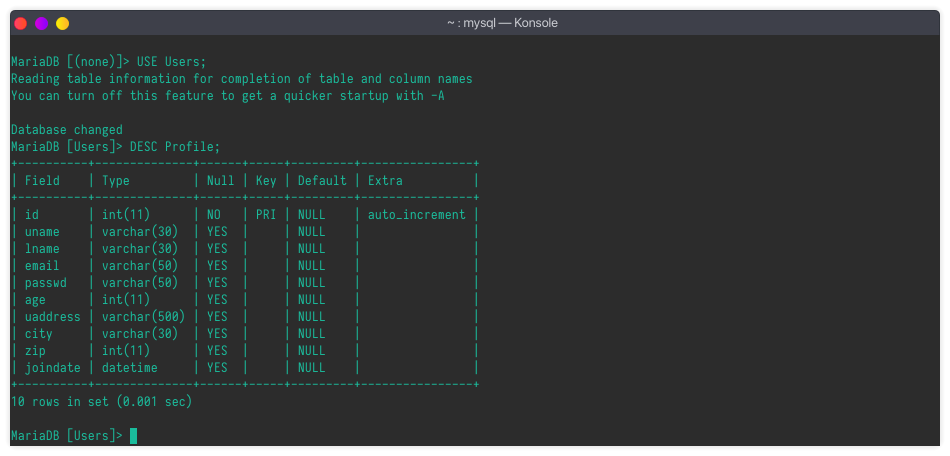
\includegraphics[width=1\textwidth]{img/p25/ss3.png}

\newpage

\subsection{Source Code}
\subsubsection{Database configuration file - config.php}
\begin{verbatim}
<?php
    /* Database configuration file */
    
    session_start();
    
    $host = "localhost";
    $user = "gokul";
    $passwd = "1821";
    $db = "Users";

    $con = mysqli_connect($host, $user, $passwd, $db);
    if(!$con){
        echo "<div class=\"error notif\">Database not found</div>";
    }
?>
\end{verbatim}
\subsubsection{Login page - index.php}
\begin{verbatim}
<?php
/* Running PHP: simple applications like login forms after setting up a 
LAMP Stack */

include("verify.php");
?>
<!DOCTYPE html>
<html>
	<head>
		<link rel="stylesheet" href="assets/style.css">
	</head>
	
	<body>
		<div id="container">
			<div class="form-container">
				<form name="login" method="POST" action="index.php">
					<h2>Log In</h2>
					<label for="username">Username:</label><br/>
					<input name="username" type="text">
					<br/>

					<label for="password">Password:</label><br/>
					<input name="password" type="password">
					<br/>

					<button type="submit" name="login-submit">Log In</button>
					<br/>
						
					<a href="signup.php">Sign up</a> for an account
				</form>
			</div>
		</div>
	</body>

</html>
\end{verbatim}

\subsubsection{User verification page - verify.php}
\begin{verbatim}
<?php
   /* Script to check the info user typed and verify or add the data to database */
   include("config.php");
   if($_SESSION["id"]){
       header("Location: welcome.php");
   }
   if(isset($_POST["login-submit"])){
       $username = mysqli_real_escape_string($con, $_POST['username']);
       $password = mysqli_real_escape_string($con, $_POST['password']);
       
       $query = mysqli_query(
           $con, 
           "SELECT id FROM Profile WHERE uname='$username' AND passwd='$password'"
       );
       $row = mysqli_fetch_array($query, MYSQLI_ASSOC);
       $found = mysqli_num_rows($query);
       if(!$found){
           echo "<div class=\"error notif\">User not found</div>";
       }
       else{
           echo "<div class=\"success notif\">Succesfully logged in.</div>";
           $_SESSION["id"] = $row["id"];
           sleep(1);
           header("Location: welcome.php");
       }
   }
   if(isset($_POST["signup-submit"])){
       $found = $_POST["username"];
       $username = mysqli_real_escape_string($con, $_POST['username']);
       $name = mysqli_real_escape_string($con, $_POST['name']);
       $email = mysqli_real_escape_string($con, $_POST['email']);
       $password = mysqli_real_escape_string($con, $_POST['password']);
       $age = mysqli_real_escape_string($con, $_POST['age']);
       $address = mysqli_real_escape_string($con, $_POST['address']);
       $city = mysqli_real_escape_string($con, $_POST['city']);
       $zip = mysqli_real_escape_string($con, $_POST['zip']);
       $date = date('Y-m-d H:i:s');
       $query = mysqli_query(
           $con,
           "INSERT INTO 
           Profile (uname, lname, email, passwd, age, uaddress, city, zip, joindate)
           VALUES ('$username', '$name', '$email', '$password', '$age', '$address',
           '$city', '$zip', '$date')"
       );
       if($query){
           $id = mysqli_insert_id($con);
           echo "<div class=\"success notif\">User added successfully</div>";
           $_SESSION["id"] = $id;
           sleep(1);
           header("Location: welcome.php");
       }
       else{
           echo "<div class=\"error notif\">Please insert valid inputs</div>";
       }
   }
?>
\end{verbatim}

\subsubsection{Signup page - signup.php}
\begin{verbatim}
<?php
/* Sign up page */

	include("verify.php");
?>

<!DOCTYPE html>
<html>
	<head>
		<link rel="stylesheet" href="assets/style.css">
	</head>
	<body>
		<div id="container">
			<div class="form-container">
				<form name="signup" method="POST" action="signup.php">
					<h2>Sign Up</h2>
					<label for="username">Username:</label><br/>
					<input name="username" type="text">
					<br/>

                    <label for="name">Name:</label><br/>
					<input name="name" type="text">
                    <br/>
                    
					<label for="email">Email:</label><br/>
					<input name="email" type="text">
					<br/>

					<label for="password">Password:</label><br/>
					<input name="password" type="password">
                    <br/>

                    <label for="age">Age:</label><br/>
                    <input name="age" type="number" max="115">
                    <br/>

                    <label for="address">Address:</label><br/>
                    <textarea name="address"></textarea><br/>

                    <label for="city">City:</label><br/>
					<input name="city" type="text">
                    <br/>

                    <label for="zip">Zip code:</label><br/>
					<input name="zip" type="number">
                    <br/>

					<button type="submit" name="signup-submit">Sign Up</button>
					<br/>
						
					<a href="index.php">Log in</a> to your account
				</form>
			</div>

		</div>
	</body>

</html>
\end{verbatim}

\subsubsection{User profile page - welcome.php}
\begin{verbatim}
<?php
    /* User profile page */
    
    include("config.php");
    $id = $_SESSION["id"];

    if(!$id){
        header("Location: index.php");
    }

    if($_GET["logout"]){
        if(session_destroy()){
            header("Location: index.php");
        }
        echo "<div class=\"success notif\">Logged out successfully/div>";
        sleep(1);
        header("Location: index.php");
    }

    $query = mysqli_query(
        $con,
        "SELECT * FROM Profile WHERE id=$id"
    );

    $row = mysqli_fetch_array($query, MYSQLI_ASSOC);
    $name = $row["lname"];
    $username = $row["uname"];
    $email = $row["email"];
    $age = $row["age"];
    $address = $row["uaddress"];
    $city = $row["city"];
    $zip = $row["zip"];
    $joindate = $row["joindate"];
?>

<!DOCTYPE html>
<html>
	<head>
		<link rel="stylesheet" href="assets/style.css">
    </head>
    
	<body>
		<div id="container">
            <div class="profile-container">
                <h1> Welcome <?php echo $username ?>,</h1>
                <h2>Your details:</h2>

                <div class="table">
                    <div class="trow">
                        <div class="tcell">Name: </div>
                        <div class="tcell"><?php echo $name ?></div>
                    </div>

                    <div class="trow">
                        <div class="tcell">Email: </div>
                        <div class="tcell"><?php echo $email ?></div>
                    </div>

                    <div class="trow">
                        <div class="tcell">Age: </div>
                        <div class="tcell"><?php echo $age ?></div>
                    </div>

                    <div class="trow">
                        <div class="tcell">Address: </div>
                        <div class="tcell"><?php echo $address ?></div>
                    </div>

                    <div class="trow">
                        <div class="tcell">City: </div>
                        <div class="tcell"><?php echo $city ?></div>
                    </div>

                    <div class="trow">
                        <div class="tcell">Zip: </div>
                        <div class="tcell"><?php echo $zip ?></div>
                    </div>
                    
                    <div class="trow">
                        <div class="tcell">Join Date: </div>
                        <div class="tcell"><?php echo $joindate ?></div>
                    </div>
                </div>
                <a href="welcome.php?logout=true">Log out</a> from your account
            </div>
		</div>
	</body>

</html>
\end{verbatim}
\newpage

\subsection{Output}
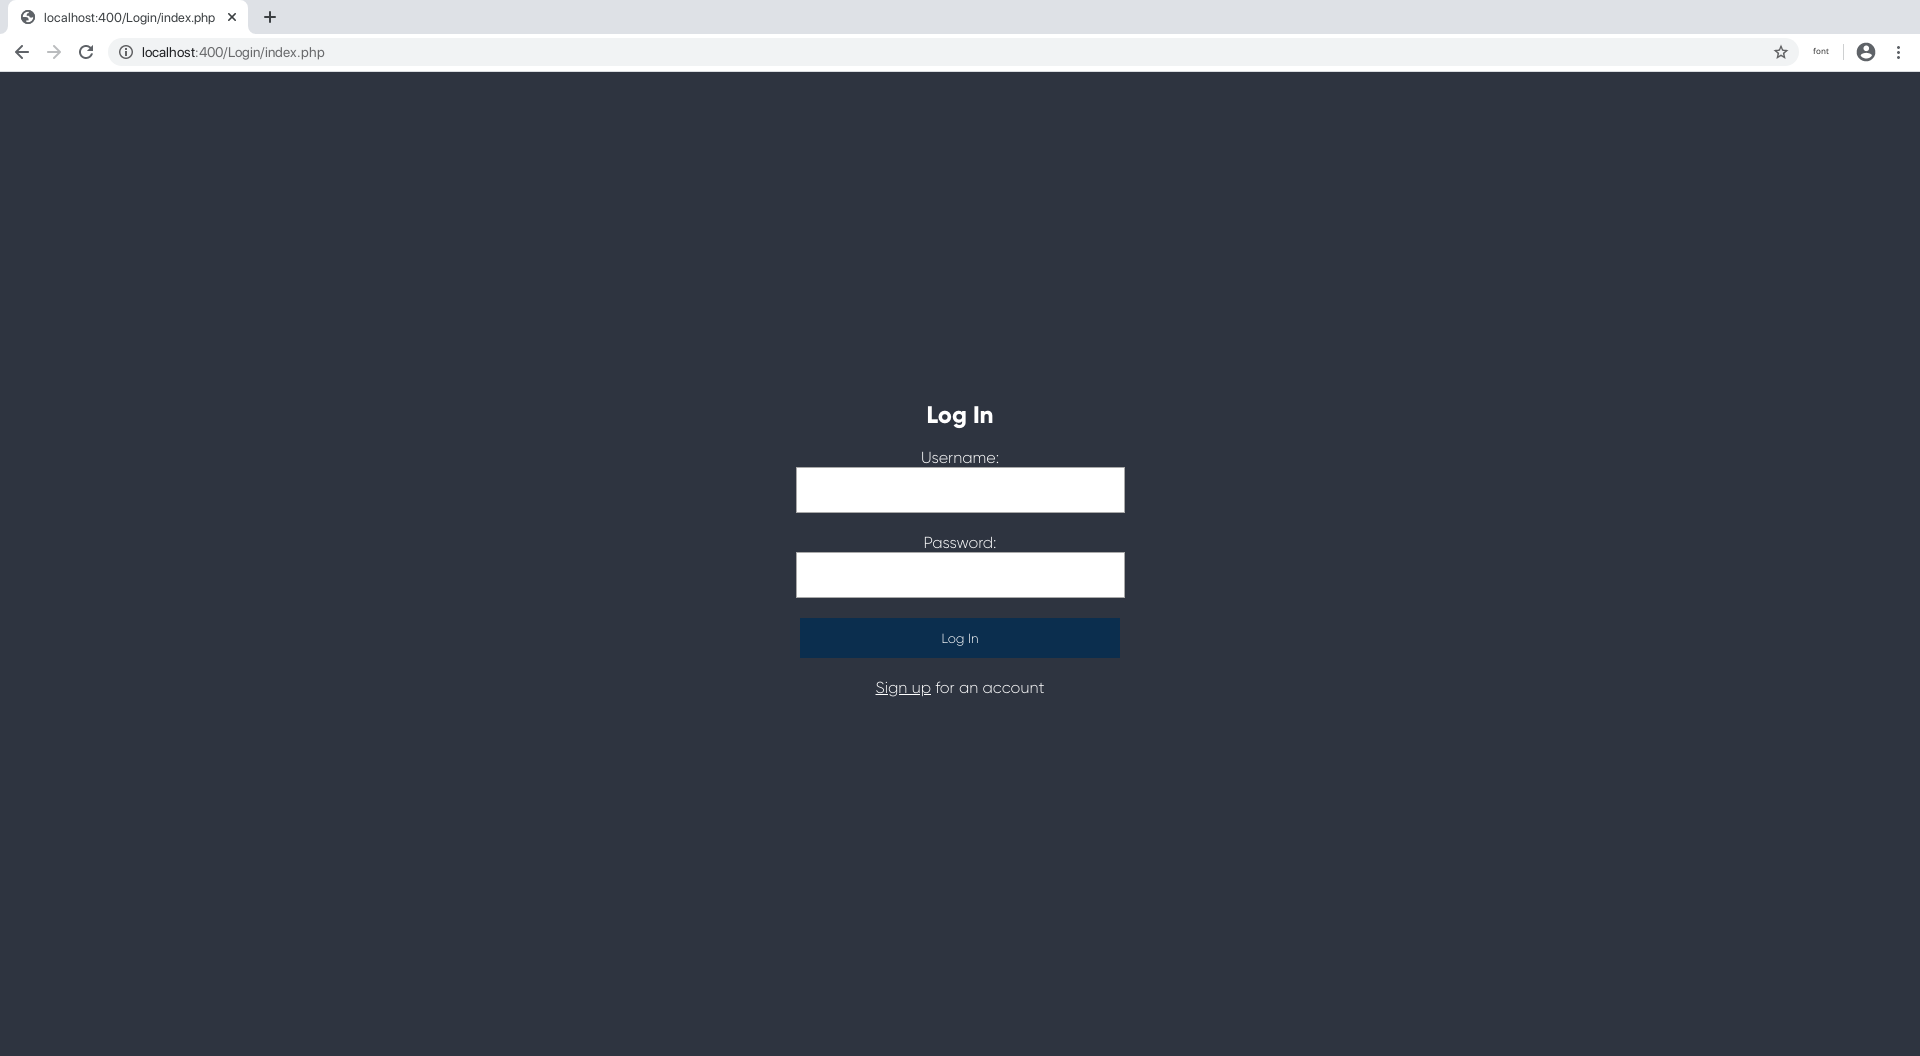
\includegraphics[width=1\textwidth]{img/p25/ss1.png}
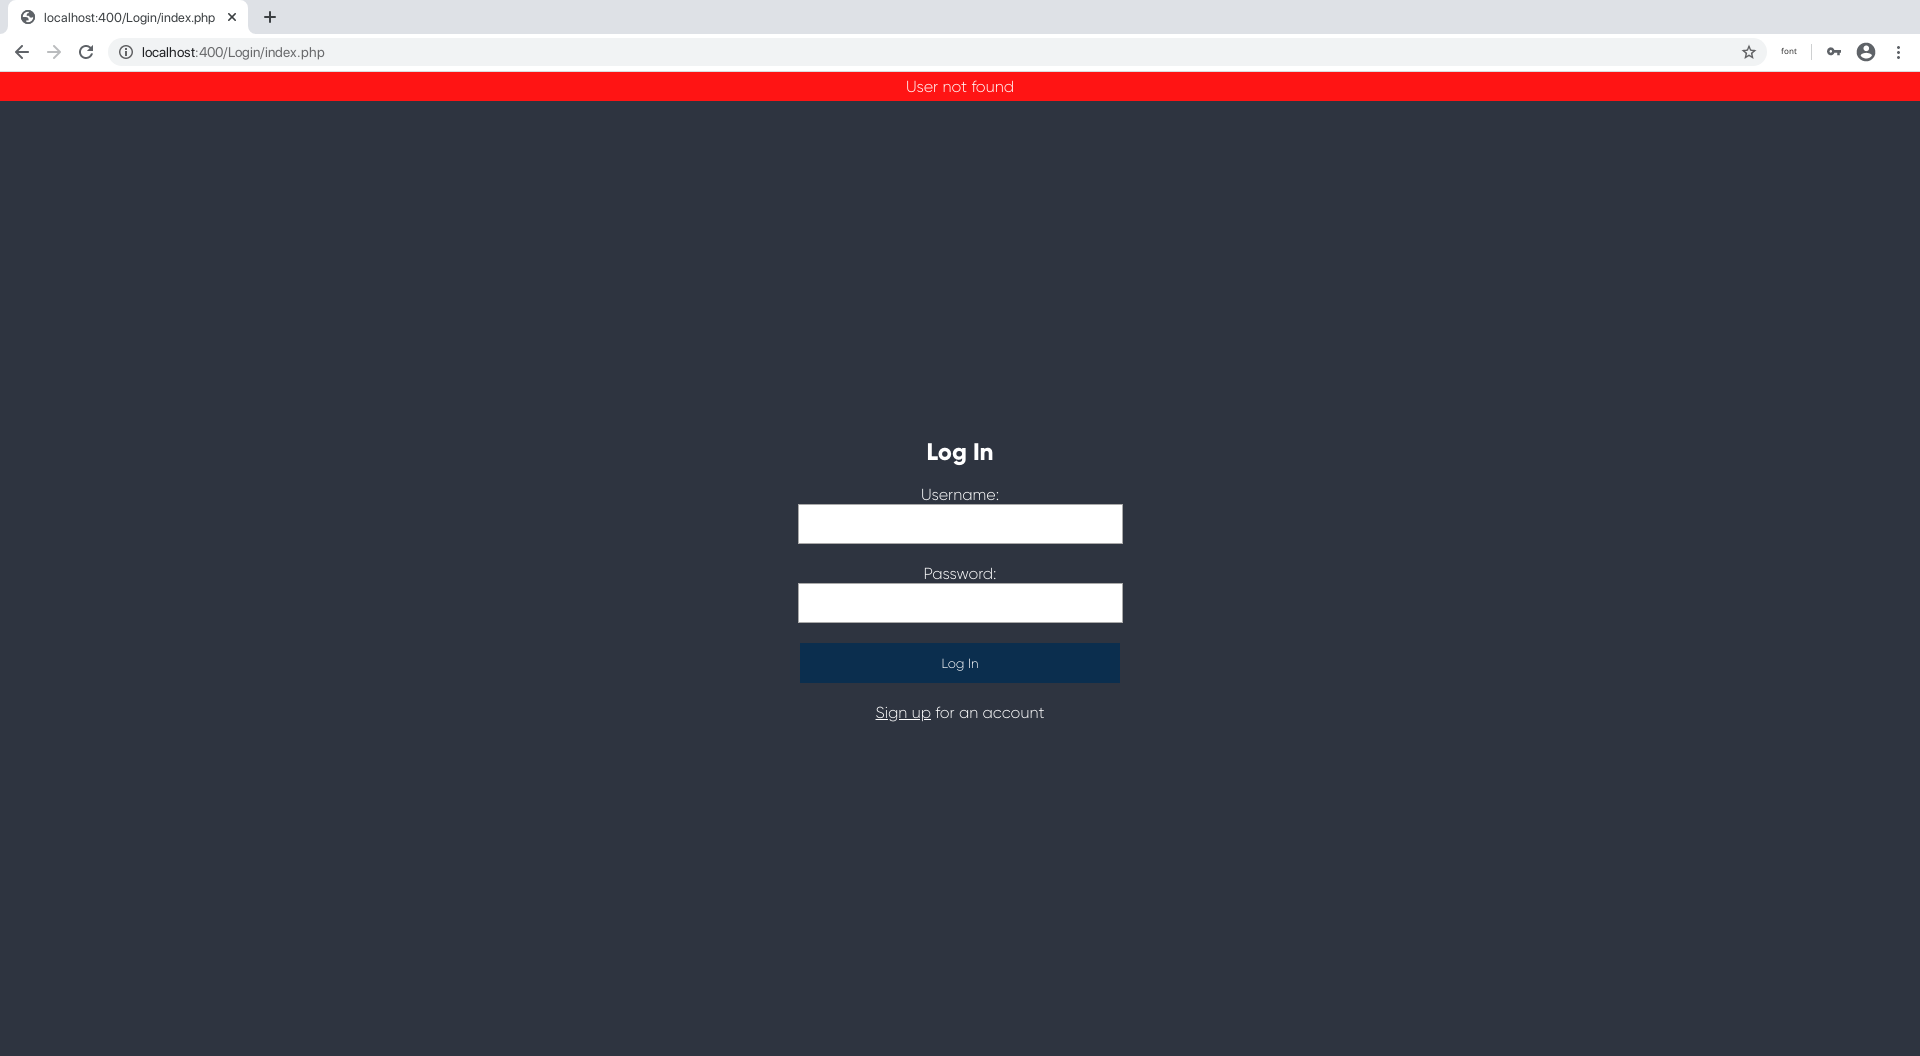
\includegraphics[width=1\textwidth]{img/p25/ss2.png}
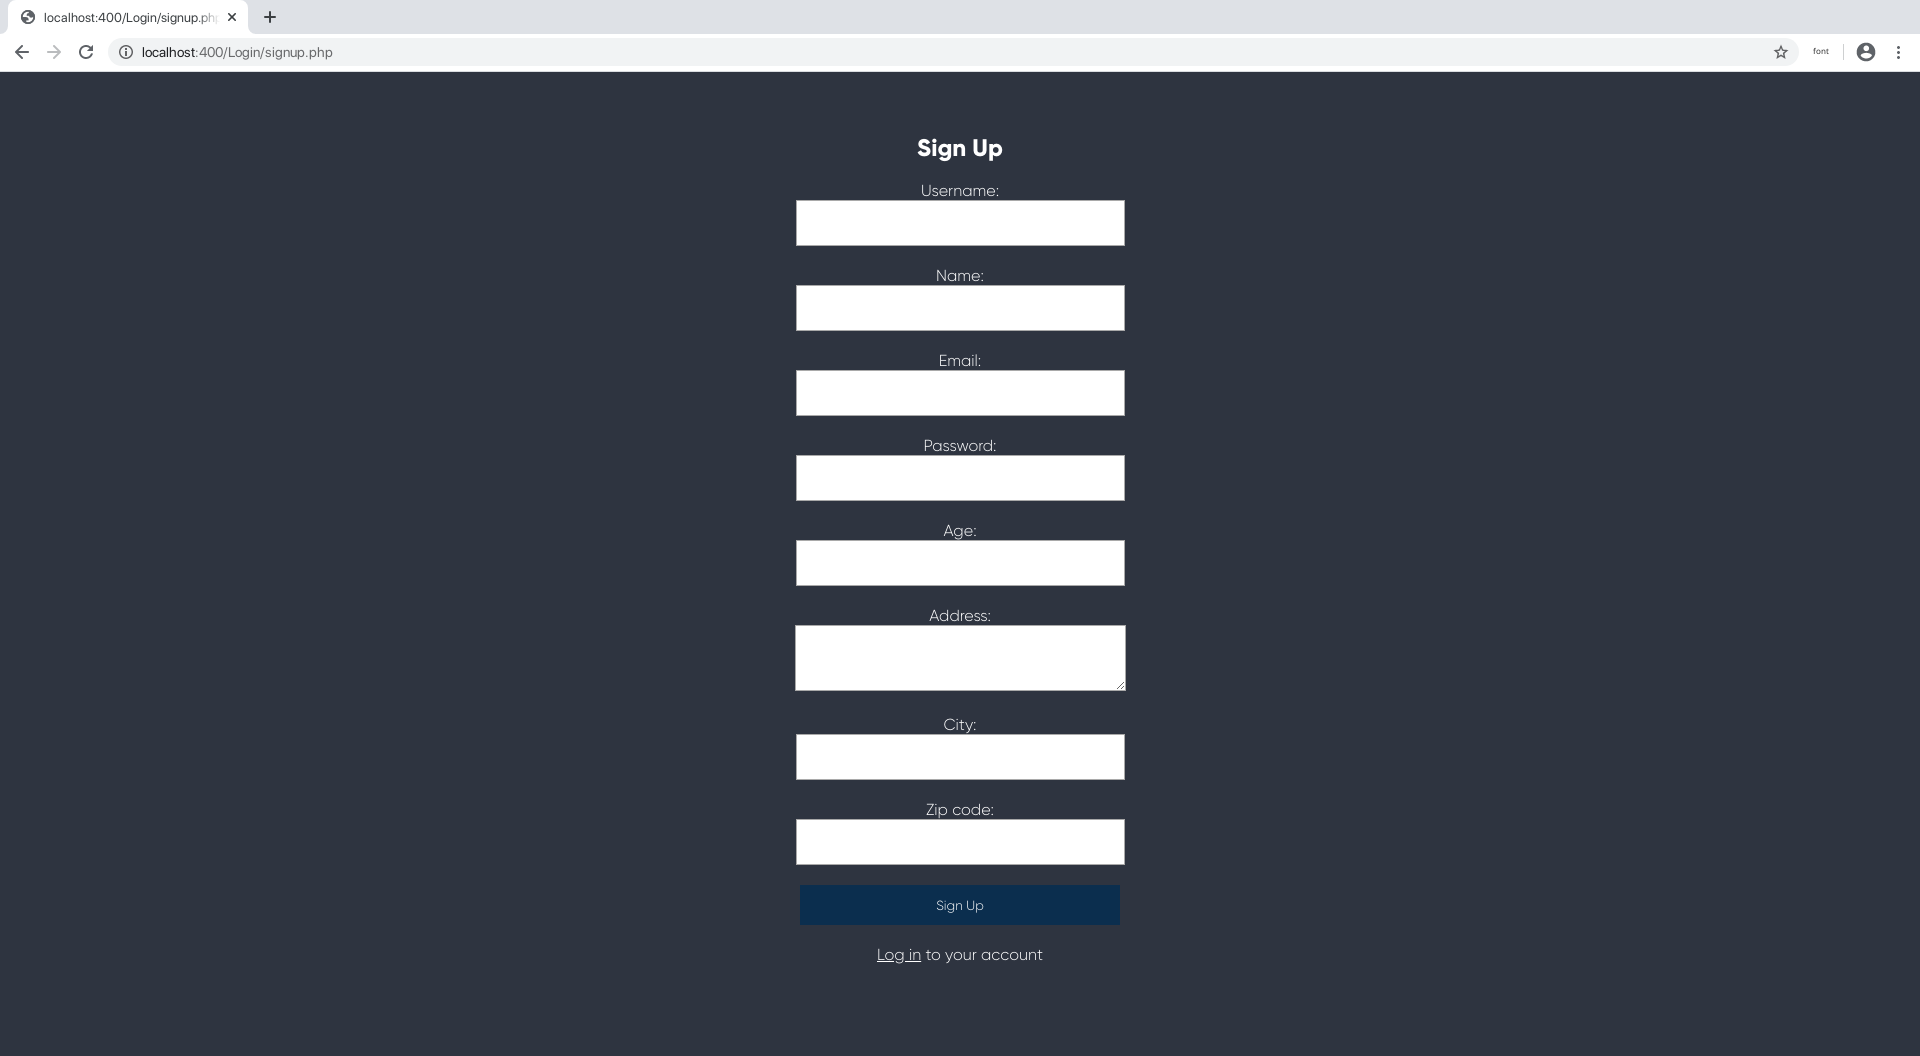
\includegraphics[width=1\textwidth]{img/p25/ss6.png}
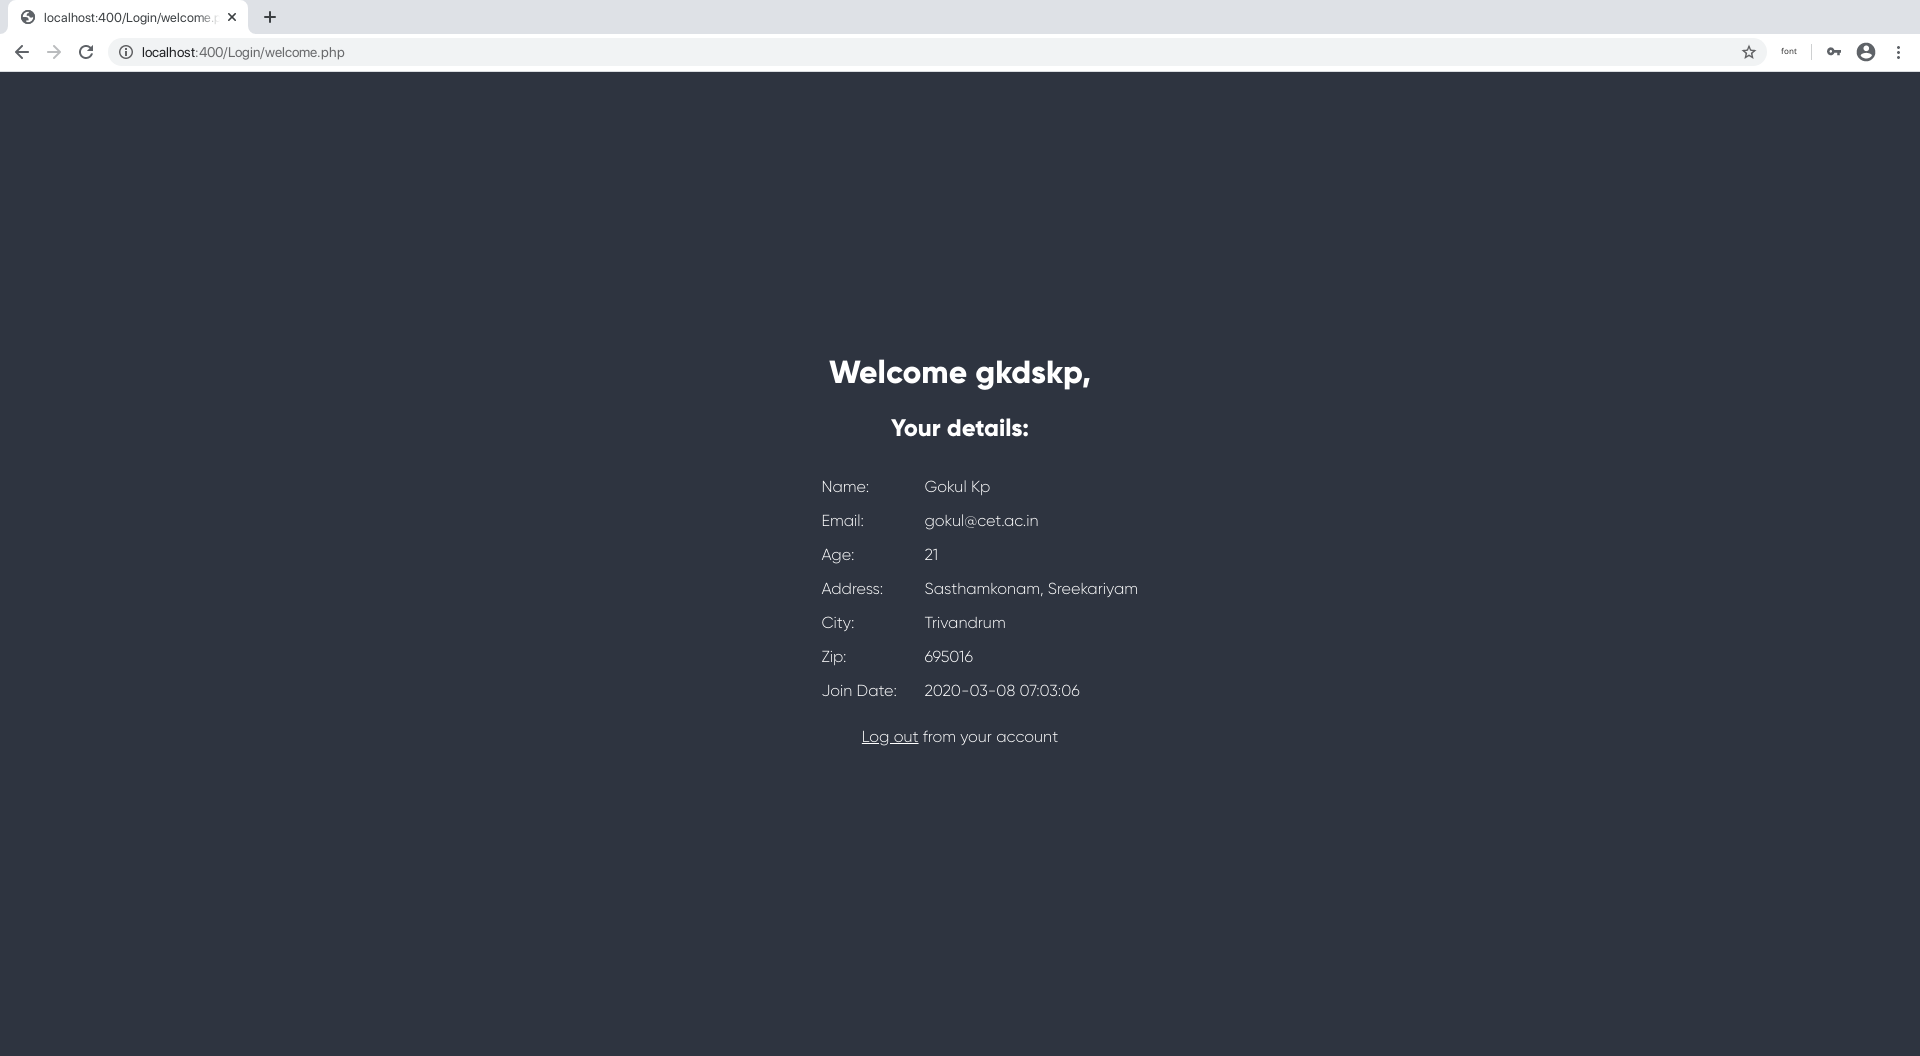
\includegraphics[width=1\textwidth]{img/p25/ss4.png}
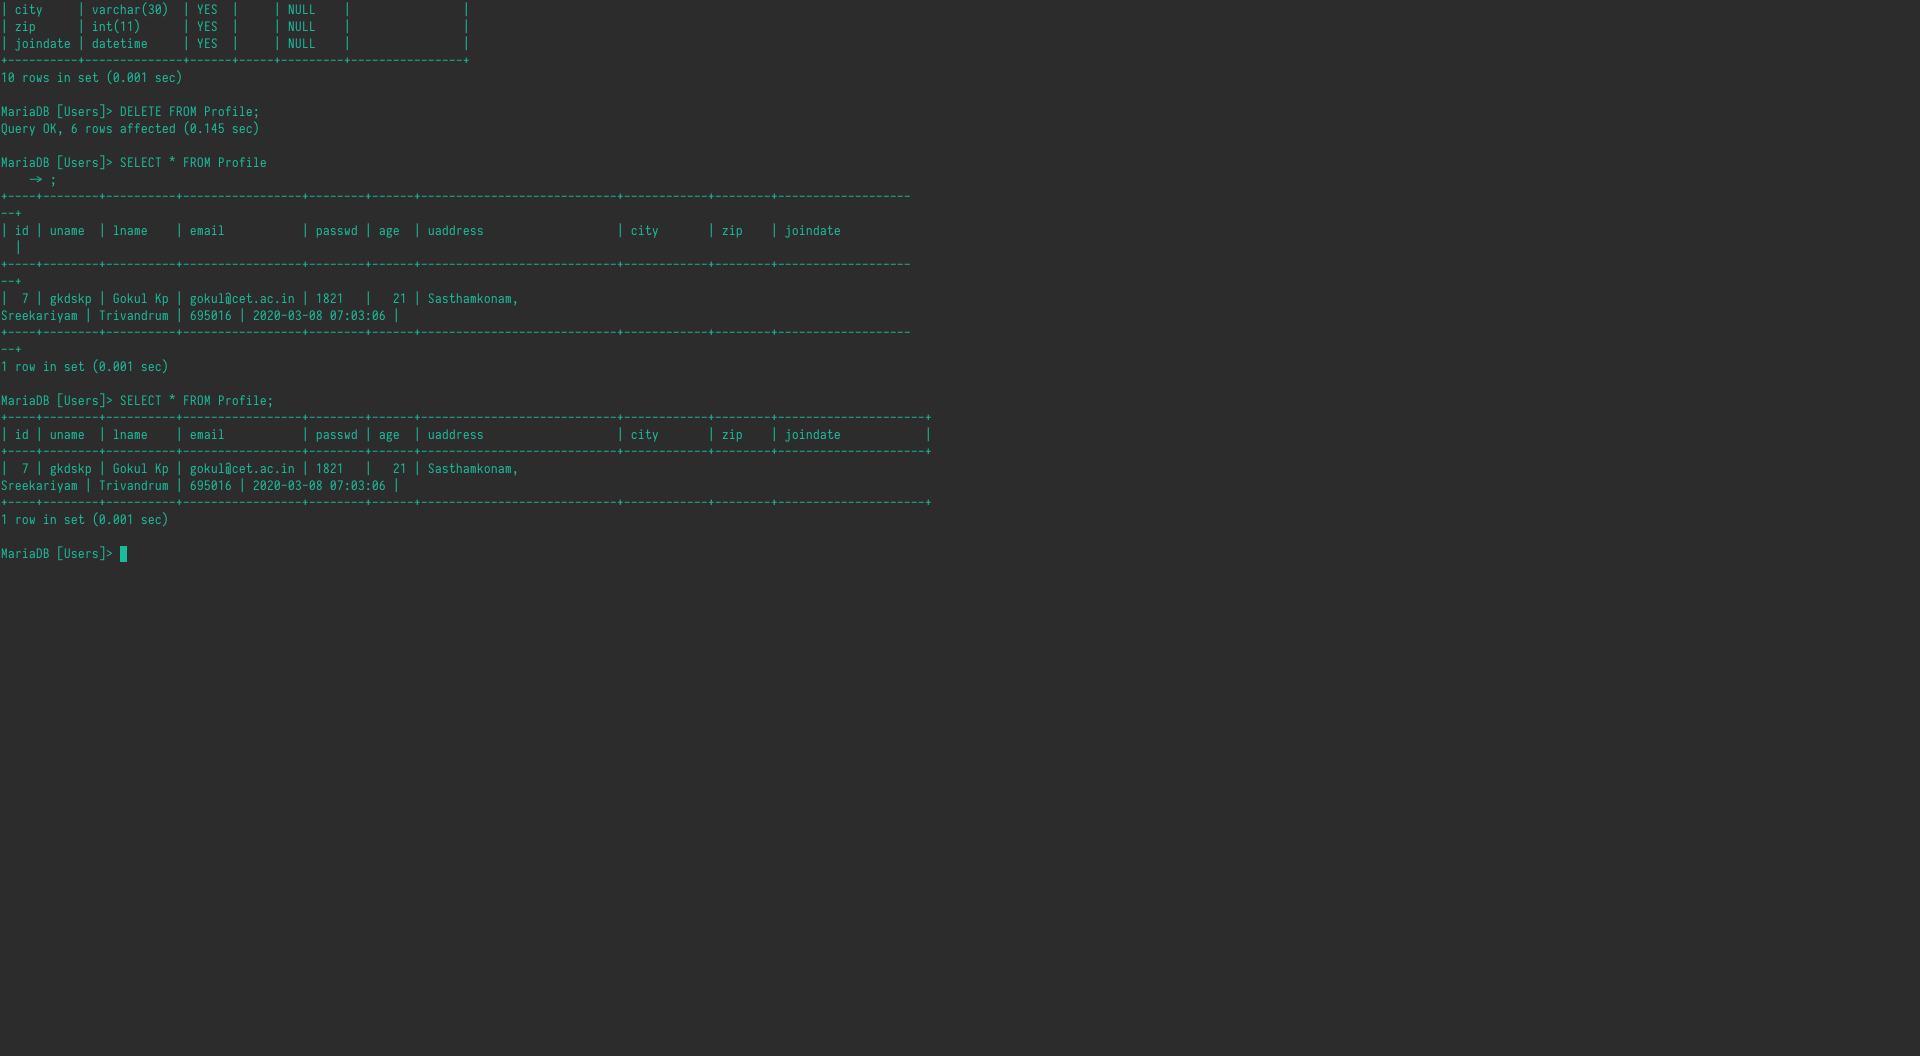
\includegraphics[width=1\textwidth]{img/p25/ss5.png}

\newpage

\subsection{Result}
LAMP Stack is installed in linux and set up. A PHP script is created
to insert user data in to a database and to verify it while logging in.
A personalised user page is displayed to each user.
\end{document}